% vim: set spell spelllang=en tw=100 :

\documentclass[letterpaper]{article}
\usepackage[pass]{geometry}

\usepackage{ijcai16}
\usepackage{times}
\usepackage{complexity}
\usepackage{microtype}
\usepackage{gnuplot-lua-tikz}
\usepackage{amsmath}
\usepackage{amssymb}
\usepackage{placeins}
\usepackage{cleveref}
\usepackage{natbib}
\usepackage{dblfloatfix}

% \usepackage{showframe}

\usetikzlibrary{decorations, decorations.pathreplacing, calc, backgrounds}

\definecolor{uofguniversityblue}{rgb}{0, 0.219608, 0.396078}

\definecolor{uofgheather}{rgb}{0.356863, 0.32549, 0.490196}
\definecolor{uofgaquamarine}{rgb}{0.603922, 0.72549, 0.678431}
\definecolor{uofgslate}{rgb}{0.309804, 0.34902, 0.380392}
\definecolor{uofgrose}{rgb}{0.823529, 0.470588, 0.709804}
\definecolor{uofgmocha}{rgb}{0.709804, 0.564706, 0.47451}
\definecolor{uofgsandstone}{rgb}{0.321569, 0.278431, 0.231373}
\definecolor{uofgforest}{rgb}{0, 0.2, 0.129412}
\definecolor{uofglawn}{rgb}{0.517647, 0.741176, 0}
\definecolor{uofgcobalt}{rgb}{0, 0.615686, 0.92549}
\definecolor{uofgturquoise}{rgb}{0, 0.709804, 0.819608}
\definecolor{uofgsunshine}{rgb}{1.0, 0.862745, 0.211765}
\definecolor{uofgpumpkin}{rgb}{1.0, 0.72549, 0.282353}
\definecolor{uofgthistle}{rgb}{0.584314, 0.070588, 0.447059}
\definecolor{uofgrust}{rgb}{0.603922, 0.227451, 0.023529}
\definecolor{uofgburgundy}{rgb}{0.490196, 0.133333, 0.223529}
\definecolor{uofgpillarbox}{rgb}{0.701961, 0.047059, 0}
\definecolor{uofglavendar}{rgb}{0.356863, 0.301961, 0.580392}

\renewcommand{\topfraction}{0.9}
\renewcommand{\bottomfraction}{0.8}
\renewcommand{\dbltopfraction}{0.9}
\renewcommand{\textfraction}{0.05}
\setcounter{dbltopnumber}{2}
\renewcommand{\floatpagefraction}{0.85}
\renewcommand{\dblfloatpagefraction}{0.85}

% cref style
\crefname{figure}{Figure}{Figures}
\Crefname{figure}{Figure}{Figures}

% http://tex.stackexchange.com/questions/22100/the-bar-and-overline-commands
\newcommand{\shortoverline}[1]{\mkern 1.5mu\overline{\mkern-1.5mu#1\mkern-1.5mu}\mkern 1.5mu}

\title{Heuristics and Really Hard Instances for Subgraph Isomorphism Problems}

% \author{Ciaran McCreesh\thanks{This work was supported by the Engineering and Physical Sciences
%     Research Council [grant number EP/K503058/1]} \and Patrick Prosser \and James Trimble \\
% University of Glasgow, Glasgow, Scotland \\
% c.mccreesh.1@research.gla.ac.uk}

\author{First Author \thanks{This work was supported by a small pile of money and a large
    electricity bill.} \and Second Author
    \and Third Author \\
Some Instituion, Somewhere, Some Country \\
anonymous@example.com}

\begin{document}

\maketitle

\begin{abstract}
    We show how to generate ``really hard'' random instances for subgraph isomorphism problems. For
    the non-induced variant, we predict and observe a phase transition between satisfiable and
    unsatisfiable instances, with a corresponding complexity peak seen in three different solvers. For
    the induced variant, much richer behaviour is observed, and constrainedness gives
    a better measure of difficulty than does proximity to a phase transition. We also discuss variable
    and value ordering heuristics, and their relationship to the expected number of solutions.
\end{abstract}

\section{Introduction}

The \emph{non-induced subgraph isomorphism problem} is to find an injective mapping from a given
pattern graph to a given target graph which preserves adjacency---in essence, we are ``finding a
copy of'' the pattern inside the target. The \emph{induced} variant of the problem additionally
requires that the mapping preserve non-adjacency, so there are no ``extra edges'' in the copy of the
pattern that we find. We illustrate both variants in \cref{figure:sip}.
Despite these problems being \NP-complete, modern practical subgraph isomorphism algorithms can
handle problem instances with many hundreds of vertices in the pattern graph, and up to ten thousand
vertices in the target graph \citep{Cordella:2004,Solnon:2010,Audemard:2014,McCreesh:2015}, leading
to successful application in areas such as computer
vision \citep{Damiand:2011,Solnon:2015}, biochemistry \citep{Giugno:2013,Carletti:2015}, and pattern
recognition \citep{Conte:2004}.

\begin{figure}[b]
    \centering
    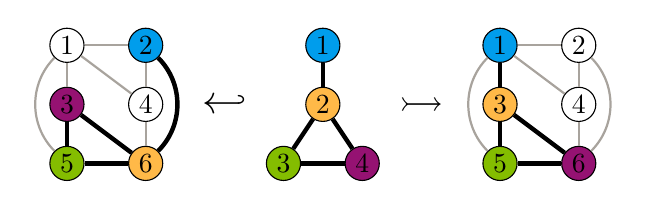
\begin{tikzpicture}[scale=0.5]
        \begin{scope}
            \node [draw, circle, fill=uofgcobalt, inner sep=1.5pt] (Na) at (1,  0) {1};
            \node [draw, circle, fill=uofgpumpkin, inner sep=1.5pt] (Nb) at (1, -1.5) {2};
            \node [draw, circle, fill=uofglawn, inner sep=1.5pt] (Nc) at (0, -3) {3};
            \node [draw, circle, fill=uofgthistle, inner sep=1.5pt] (Nd) at (2, -3) {4};

            \draw [ultra thick] (Na) -- (Nb);
            \draw [ultra thick] (Nb) -- (Nc);
            \draw [ultra thick] (Nc) -- (Nd);
            \draw [ultra thick] (Nb) -- (Nd);

            \node [draw, circle, fill=uofgcobalt, inner sep=1.5pt] (N1) at (5.5,  0) {1};
            \node [draw, circle, fill=white, inner sep=1.5pt] (N2) at (7.5,  0) {2};
            \node [draw, circle, fill=uofgpumpkin, inner sep=1.5pt] (N3) at (5.5, -1.5) {3};
            \node [draw, circle, fill=white, inner sep=1.5pt] (N4) at (7.5, -1.5) {4};
            \node [draw, circle, fill=uofglawn, inner sep=1.5pt] (N5) at (5.5, -3) {5};
            \node [draw, circle, fill=uofgthistle, inner sep=1.5pt] (N6) at (7.5, -3) {6};

            \draw [thick, color=uofgsandstone!50] (N1) -- (N2);
            \draw [ultra thick] (N1) -- (N3);
            \draw [thick, color=uofgsandstone!50] (N1) -- (N4);
            \draw [thick, color=uofgsandstone!50] (N2) -- (N4);
            \draw [ultra thick] (N3) -- (N5);
            \draw [ultra thick] (N3) -- (N6);
            \draw [thick, color=uofgsandstone!50] (N4) -- (N6);
            \draw [ultra thick] (N5) -- (N6);
            \draw [thick, color=uofgsandstone!50] (N2) to [in=45, out=315] (N6);
            \draw [thick, color=uofgsandstone!50] (N1) to [in=135, out=225] (N5);

            \node [draw, circle, fill=white, inner sep=1.5pt] (M1) at (-5.5,  0) {1};
            \node [draw, circle, fill=uofgcobalt, inner sep=1.5pt] (M2) at (-3.5,  0) {2};
            \node [draw, circle, fill=uofgthistle, inner sep=1.5pt] (M3) at (-5.5, -1.5) {3};
            \node [draw, circle, fill=white, inner sep=1.5pt] (M4) at (-3.5, -1.5) {4};
            \node [draw, circle, fill=uofglawn, inner sep=1.5pt] (M5) at (-5.5, -3) {5};
            \node [draw, circle, fill=uofgpumpkin, inner sep=1.5pt] (M6) at (-3.5, -3) {6};

            \draw [thick, color=uofgsandstone!50] (M1) -- (M2);
            \draw [thick, color=uofgsandstone!50] (M1) -- (M3);
            \draw [thick, color=uofgsandstone!50] (M1) -- (M4);
            \draw [thick, color=uofgsandstone!50] (M2) -- (M4);
            \draw [ultra thick] (M3) -- (M5);
            \draw [ultra thick] (M3) -- (M6);
            \draw [thick, color=uofgsandstone!50] (M4) -- (M6);
            \draw [ultra thick] (M5) -- (M6);
            \draw [ultra thick] (M2) to [in=45, out=315] (M6);
            \draw [thick, color=uofgsandstone!50] (M1) to [in=135, out=225] (M5);

            \node [anchor=center, font=\Large] (A1) at (-1.5, -1.5) { $\hookleftarrow$ };
            \node [anchor=center, font=\Large] (A2) at ( 3.5, -1.5) { $\rightarrowtail$ };
        \end{scope}
    \end{tikzpicture}\\[0.75cm]
    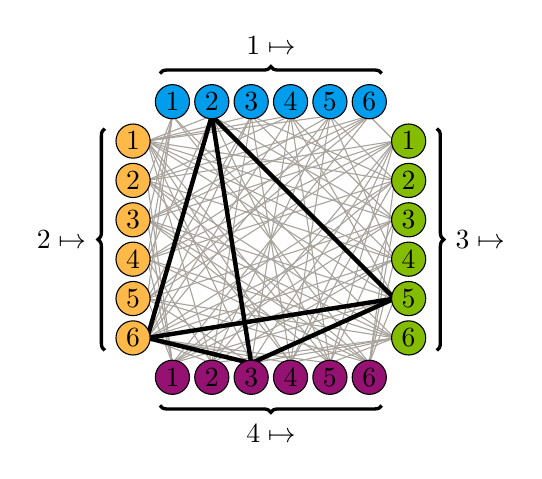
\begin{tikzpicture}[scale=0.5]
        \begin{scope}
            \foreach \n in {1, ..., 6}{
                \node [draw, circle, fill=uofgcobalt, inner sep=1.5pt] (N1\n) at (\n, 0) {\n};
            }

            \draw [decorate, decoration={brace, raise=0.2cm}, very thick] (N11.north west) -- (N16.north
                east) node [midway, above=0.3cm] { $1 \mapsto$ };

            \foreach \n in {1, ..., 6}{
                \node [draw, circle, fill=uofgpumpkin, inner sep=1.5pt] (N2\n) at (0, -\n) {\n};
            }

            \draw [decorate, decoration={brace, raise=0.2cm, mirror}, very thick] (N21.north west) --
                (N26.south west) node [midway, left=0.3cm] { $2 \mapsto$ };

            \foreach \n in {1, ..., 6}{
                \node [draw, circle, fill=uofglawn, inner sep=1.5pt] (N3\n) at (7, -\n) {\n};
            }

            \draw [decorate, decoration={brace, raise=0.2cm}, very thick] (N31.north east) -- (N36.south
                east) node [midway, right=0.3cm] { $3 \mapsto$ };

            \foreach \n in {1, ..., 6}{
                \node [draw, circle, fill=uofgthistle, inner sep=1.5pt] (N4\n) at (\n, -7) {\n};
            }

            \draw [decorate, decoration={brace, raise=0.2cm, mirror}, very thick] (N41.south west) --
                (N46.south east) node [midway, below=0.3cm] { $4 \mapsto$ };

            \begin{scope}[on background layer]
                \draw [color=uofgsandstone!50] ($(N11)!0.8!(N11.south)$) -- ($(N22)!0.8!(N22.east)$);
                \draw [color=uofgsandstone!50] ($(N11)!0.8!(N11.south)$) -- ($(N23)!0.8!(N23.east)$);
                \draw [color=uofgsandstone!50] ($(N11)!0.8!(N11.south)$) -- ($(N24)!0.8!(N24.east)$);
                \draw [color=uofgsandstone!50] ($(N11)!0.8!(N11.south)$) -- ($(N25)!0.8!(N25.east)$);
                \draw [color=uofgsandstone!50] ($(N11)!0.8!(N11.south)$) -- ($(N36)!0.8!(N36.west)$);
                \draw [color=uofgsandstone!50] ($(N11)!0.8!(N11.south)$) -- ($(N46)!0.8!(N46.north)$);
                \draw [color=uofgsandstone!50] ($(N21)!0.8!(N21.east)$) -- ($(N12)!0.8!(N12.south)$);
                \draw [color=uofgsandstone!50] ($(N21)!0.8!(N21.east)$) -- ($(N32)!0.8!(N32.west)$);
                \draw [color=uofgsandstone!50] ($(N21)!0.8!(N21.east)$) -- ($(N42)!0.8!(N42.north)$);
                \draw [color=uofgsandstone!50] ($(N21)!0.8!(N21.east)$) -- ($(N13)!0.8!(N13.south)$);
                \draw [color=uofgsandstone!50] ($(N21)!0.8!(N21.east)$) -- ($(N33)!0.8!(N33.west)$);
                \draw [color=uofgsandstone!50] ($(N21)!0.8!(N21.east)$) -- ($(N43)!0.8!(N43.north)$);
                \draw [color=uofgsandstone!50] ($(N21)!0.8!(N21.east)$) -- ($(N14)!0.8!(N14.south)$);
                \draw [color=uofgsandstone!50] ($(N21)!0.8!(N21.east)$) -- ($(N34)!0.8!(N34.west)$);
                \draw [color=uofgsandstone!50] ($(N21)!0.8!(N21.east)$) -- ($(N44)!0.8!(N44.north)$);
                \draw [color=uofgsandstone!50] ($(N21)!0.8!(N21.east)$) -- ($(N15)!0.8!(N15.south)$);
                \draw [color=uofgsandstone!50] ($(N21)!0.8!(N21.east)$) -- ($(N35)!0.8!(N35.west)$);
                \draw [color=uofgsandstone!50] ($(N21)!0.8!(N21.east)$) -- ($(N45)!0.8!(N45.north)$);
                \draw [color=uofgsandstone!50] ($(N31)!0.8!(N31.west)$) -- ($(N22)!0.8!(N22.east)$);
                \draw [color=uofgsandstone!50] ($(N31)!0.8!(N31.west)$) -- ($(N42)!0.8!(N42.north)$);
                \draw [color=uofgsandstone!50] ($(N31)!0.8!(N31.west)$) -- ($(N23)!0.8!(N23.east)$);
                \draw [color=uofgsandstone!50] ($(N31)!0.8!(N31.west)$) -- ($(N43)!0.8!(N43.north)$);
                \draw [color=uofgsandstone!50] ($(N31)!0.8!(N31.west)$) -- ($(N24)!0.8!(N24.east)$);
                \draw [color=uofgsandstone!50] ($(N31)!0.8!(N31.west)$) -- ($(N44)!0.8!(N44.north)$);
                \draw [color=uofgsandstone!50] ($(N31)!0.8!(N31.west)$) -- ($(N25)!0.8!(N25.east)$);
                \draw [color=uofgsandstone!50] ($(N31)!0.8!(N31.west)$) -- ($(N45)!0.8!(N45.north)$);
                \draw [color=uofgsandstone!50] ($(N31)!0.8!(N31.west)$) -- ($(N16)!0.8!(N16.south)$);
                \draw [color=uofgsandstone!50] ($(N41)!0.8!(N41.north)$) -- ($(N22)!0.8!(N22.east)$);
                \draw [color=uofgsandstone!50] ($(N41)!0.8!(N41.north)$) -- ($(N32)!0.8!(N32.west)$);
                \draw [color=uofgsandstone!50] ($(N41)!0.8!(N41.north)$) -- ($(N23)!0.8!(N23.east)$);
                \draw [color=uofgsandstone!50] ($(N41)!0.8!(N41.north)$) -- ($(N33)!0.8!(N33.west)$);
                \draw [color=uofgsandstone!50] ($(N41)!0.8!(N41.north)$) -- ($(N24)!0.8!(N24.east)$);
                \draw [color=uofgsandstone!50] ($(N41)!0.8!(N41.north)$) -- ($(N34)!0.8!(N34.west)$);
                \draw [color=uofgsandstone!50] ($(N41)!0.8!(N41.north)$) -- ($(N25)!0.8!(N25.east)$);
                \draw [color=uofgsandstone!50] ($(N41)!0.8!(N41.north)$) -- ($(N35)!0.8!(N35.west)$);
                \draw [color=uofgsandstone!50] ($(N41)!0.8!(N41.north)$) -- ($(N16)!0.8!(N16.south)$);
                \draw [color=uofgsandstone!50] ($(N12)!0.8!(N12.south)$) -- ($(N33)!0.8!(N33.west)$);
                \draw [color=uofgsandstone!50] ($(N12)!0.8!(N12.south)$) -- ($(N24)!0.8!(N24.east)$);
                \draw [color=uofgsandstone!50] ($(N12)!0.8!(N12.south)$) -- ($(N45)!0.8!(N45.north)$);
                \draw [color=uofgsandstone!50] ($(N22)!0.8!(N22.east)$) -- ($(N14)!0.8!(N14.south)$);
                \draw [color=uofgsandstone!50] ($(N22)!0.8!(N22.east)$) -- ($(N34)!0.8!(N34.west)$);
                \draw [color=uofgsandstone!50] ($(N22)!0.8!(N22.east)$) -- ($(N44)!0.8!(N44.north)$);
                \draw [color=uofgsandstone!50] ($(N22)!0.8!(N22.east)$) -- ($(N16)!0.8!(N16.south)$);
                \draw [color=uofgsandstone!50] ($(N22)!0.8!(N22.east)$) -- ($(N36)!0.8!(N36.west)$);
                \draw [color=uofgsandstone!50] ($(N22)!0.8!(N22.east)$) -- ($(N46)!0.8!(N46.north)$);
                \draw [color=uofgsandstone!50] ($(N32)!0.8!(N32.west)$) -- ($(N13)!0.8!(N13.south)$);
                \draw [color=uofgsandstone!50] ($(N32)!0.8!(N32.west)$) -- ($(N24)!0.8!(N24.east)$);
                \draw [color=uofgsandstone!50] ($(N32)!0.8!(N32.west)$) -- ($(N44)!0.8!(N44.north)$);
                \draw [color=uofgsandstone!50] ($(N32)!0.8!(N32.west)$) -- ($(N15)!0.8!(N15.south)$);
                \draw [color=uofgsandstone!50] ($(N32)!0.8!(N32.west)$) -- ($(N26)!0.8!(N26.east)$);
                \draw [color=uofgsandstone!50] ($(N32)!0.8!(N32.west)$) -- ($(N46)!0.8!(N46.north)$);
                \draw [color=uofgsandstone!50] ($(N42)!0.8!(N42.north)$) -- ($(N13)!0.8!(N13.south)$);
                \draw [color=uofgsandstone!50] ($(N42)!0.8!(N42.north)$) -- ($(N24)!0.8!(N24.east)$);
                \draw [color=uofgsandstone!50] ($(N42)!0.8!(N42.north)$) -- ($(N34)!0.8!(N34.west)$);
                \draw [color=uofgsandstone!50] ($(N42)!0.8!(N42.north)$) -- ($(N15)!0.8!(N15.south)$);
                \draw [color=uofgsandstone!50] ($(N42)!0.8!(N42.north)$) -- ($(N26)!0.8!(N26.east)$);
                \draw [color=uofgsandstone!50] ($(N42)!0.8!(N42.north)$) -- ($(N36)!0.8!(N36.west)$);
                \draw [color=uofgsandstone!50] ($(N13)!0.8!(N13.south)$) -- ($(N34)!0.8!(N34.west)$);
                \draw [color=uofgsandstone!50] ($(N13)!0.8!(N13.south)$) -- ($(N44)!0.8!(N44.north)$);
                \draw [color=uofgsandstone!50] ($(N13)!0.8!(N13.south)$) -- ($(N25)!0.8!(N25.east)$);
                \draw [color=uofgsandstone!50] ($(N13)!0.8!(N13.south)$) -- ($(N26)!0.8!(N26.east)$);
                \draw [color=uofgsandstone!50] ($(N23)!0.8!(N23.east)$) -- ($(N15)!0.8!(N15.south)$);
                \draw [color=uofgsandstone!50] ($(N23)!0.8!(N23.east)$) -- ($(N35)!0.8!(N35.west)$);
                \draw [color=uofgsandstone!50] ($(N23)!0.8!(N23.east)$) -- ($(N45)!0.8!(N45.north)$);
                \draw [color=uofgsandstone!50] ($(N23)!0.8!(N23.east)$) -- ($(N16)!0.8!(N16.south)$);
                \draw [color=uofgsandstone!50] ($(N23)!0.8!(N23.east)$) -- ($(N36)!0.8!(N36.west)$);
                \draw [color=uofgsandstone!50] ($(N23)!0.8!(N23.east)$) -- ($(N46)!0.8!(N46.north)$);
                \draw [color=uofgsandstone!50] ($(N33)!0.8!(N33.west)$) -- ($(N14)!0.8!(N14.south)$);
                \draw [color=uofgsandstone!50] ($(N33)!0.8!(N33.west)$) -- ($(N25)!0.8!(N25.east)$);
                \draw [color=uofgsandstone!50] ($(N33)!0.8!(N33.west)$) -- ($(N45)!0.8!(N45.north)$);
                \draw [color=uofgsandstone!50] ($(N33)!0.8!(N33.west)$) -- ($(N26)!0.8!(N26.east)$);
                \draw [color=uofgsandstone!50] ($(N33)!0.8!(N33.west)$) -- ($(N46)!0.8!(N46.north)$);
                \draw [color=uofgsandstone!50] ($(N43)!0.8!(N43.north)$) -- ($(N14)!0.8!(N14.south)$);
                \draw [color=uofgsandstone!50] ($(N43)!0.8!(N43.north)$) -- ($(N25)!0.8!(N25.east)$);
                \draw [color=uofgsandstone!50] ($(N43)!0.8!(N43.north)$) -- ($(N36)!0.8!(N36.west)$);
                \draw [color=uofgsandstone!50] ($(N14)!0.8!(N14.south)$) -- ($(N35)!0.8!(N35.west)$);
                \draw [color=uofgsandstone!50] ($(N14)!0.8!(N14.south)$) -- ($(N45)!0.8!(N45.north)$);
                \draw [color=uofgsandstone!50] ($(N14)!0.8!(N14.south)$) -- ($(N26)!0.8!(N26.east)$);
                \draw [color=uofgsandstone!50] ($(N24)!0.8!(N24.east)$) -- ($(N16)!0.8!(N16.south)$);
                \draw [color=uofgsandstone!50] ($(N24)!0.8!(N24.east)$) -- ($(N36)!0.8!(N36.west)$);
                \draw [color=uofgsandstone!50] ($(N24)!0.8!(N24.east)$) -- ($(N46)!0.8!(N46.north)$);
                \draw [color=uofgsandstone!50] ($(N34)!0.8!(N34.west)$) -- ($(N15)!0.8!(N15.south)$);
                \draw [color=uofgsandstone!50] ($(N34)!0.8!(N34.west)$) -- ($(N26)!0.8!(N26.east)$);
                \draw [color=uofgsandstone!50] ($(N34)!0.8!(N34.west)$) -- ($(N46)!0.8!(N46.north)$);
                \draw [color=uofgsandstone!50] ($(N44)!0.8!(N44.north)$) -- ($(N15)!0.8!(N15.south)$);
                \draw [color=uofgsandstone!50] ($(N44)!0.8!(N44.north)$) -- ($(N26)!0.8!(N26.east)$);
                \draw [color=uofgsandstone!50] ($(N44)!0.8!(N44.north)$) -- ($(N36)!0.8!(N36.west)$);
                \draw [color=uofgsandstone!50] ($(N15)!0.8!(N15.south)$) -- ($(N26)!0.8!(N26.east)$);
                \draw [color=uofgsandstone!50] ($(N25)!0.8!(N25.east)$) -- ($(N16)!0.8!(N16.south)$);
                \draw [color=uofgsandstone!50] ($(N25)!0.8!(N25.east)$) -- ($(N36)!0.8!(N36.west)$);
                \draw [color=uofgsandstone!50] ($(N25)!0.8!(N25.east)$) -- ($(N46)!0.8!(N46.north)$);
                \draw [color=uofgsandstone!50] ($(N35)!0.8!(N35.west)$) -- ($(N46)!0.8!(N46.north)$);
                \draw [color=uofgsandstone!50] ($(N45)!0.8!(N45.north)$) -- ($(N26)!0.8!(N26.east)$);
                \draw [color=uofgsandstone!50] ($(N45)!0.8!(N45.north)$) -- ($(N36)!0.8!(N36.west)$);
                \draw [ultra thick] ($(N12)!0.8!(N12.south)$) -- ($(N43)!0.8!(N43.north)$);
                \draw [ultra thick] ($(N12)!0.8!(N12.south)$) -- ($(N35)!0.8!(N35.west)$);
                \draw [ultra thick] ($(N12)!0.8!(N12.south)$) -- ($(N26)!0.8!(N26.east)$);
                \draw [ultra thick] ($(N43)!0.8!(N43.north)$) -- ($(N35)!0.8!(N35.west)$);
                \draw [ultra thick] ($(N43)!0.8!(N43.north)$) -- ($(N26)!0.8!(N26.east)$);
                \draw [ultra thick] ($(N35)!0.8!(N35.west)$) -- ($(N26)!0.8!(N26.east)$);
            \end{scope}
        \end{scope}
    \end{tikzpicture}

    \caption{On top, there is a non-induced isomorphism from the pattern graph, in the center, to the target
    on the right, mapping vertex 1 to 1, 2 to 3, 3 to 5 and 4 to 6. This is not an induced
    isomorphism, since there is an edge between 1 and 5 in the target but not between 1 and 3 in the
    pattern. The mapping from the pattern to the (same) target on the left, sending 1 to 2, 2 to 6, 3 to
    5 and 4 to 3, is both non-induced and induced.
    Below, the association graph encoding for the induced version: the highlighted clique
    corresponds to the same mapping.}
    \label{figure:sip}
\end{figure}

However, these algorithms cannot handle \emph{arbitrary} instances of this size. The experimental
evaluations of these algorithms were performed using a mix of real-world graphs, graphs that encode
biochemistry and computer vision problems, and randomly generated graph pairs. Using random
instances to evaluate algorithm behaviour can be beneficial, because it provides a way of generating
many instances cheaply, and reduces the risk of over-fitting when tuning design parameters. The
random instances used in each case came from common datasets \citep{DeSanto:2003,Zampelli:2010},
which were generated by taking a random subgraph of a random graph (using various models, including
Erd\H{o}s-R\'enyi, scale-free, bounded degree, and meshes) and permuting the vertices. Such
instances are guaranteed to be satisfiable---\citet{Anton:2009} exploited this property to create
large sets of random satisfiable boolean satisfiability instances.  However, since this has been the
only approach used to generate random subgraph isomorphism instances, existing benchmark suites
contain relatively few non-trivial unsatisfiable instances, and the satisfiable instances tend to be
computationally fairly easy, with most of the difficulty being in dealing with the size of the
model. This has lead to bias in algorithm design, to the extent that some proposed techniques will
\emph{only} work on satisfiable instances \citet{Battiti:2007}.

%%% The lack of unsatisfiable instances cannot be addressed by using a pattern graph from one of the
%%% random suites with the ``wrong'' target graph: this tends to give either a trivially unsatisfiable
%%% instance, or a satisfiable instance. (In particular, it is \emph{not} the case that a relatively
%%% small random graph is unlikely to appear in a larger random graph.)

Here we present and evaluate a new method for creating random pattern/target pairs. This method
generates both satisfiable and unsatisfiable instances, and can produce computationally challenging
instances with only a few tens of vertices in the pattern, and 150 vertices in the target. Our work
builds upon the phase transition phenomena observed in satisfiability and graph colouring problems
first described by \citet{Cheeseman:1991} and \citet{Mitchell:1992}.  For subgraph isomorphism we
identify three relevant control parameters: we can independently alter the edge probability of the
pattern graph, the edge probability of the target graph, and the relative orders (number of
vertices) of the pattern and target graphs.  For non-induced isomorphisms, with the correct choice
of parameters we see results very similar to those observed with boolean satisfiability problems:
there is a phase transition (whose location we can predict) from satisfiable to unsatisfiable,
we see a solver-independent complexity peak occur near this phase transition, and understanding this
behaviour helps us to select variable and value ordering heuristics.

For certain choices of parameters for induced isomorphisms, there are two phase transitions, going
from satisfiable to unsatisfiable, and then from unsatisfiable back to satisfiable. Again, when
going from satisfiable to unsatisfiable (from either direction), instances go from being trivial to
really hard to solve. However, each of the three solvers we tested also finds the central
unsatisfiable region to be hard, despite it not being near a phase transition. To show that this is
not a simple weakness of current subgraph isomorphism algorithms, we verify that this region is also
hard when using a pseudo-boolean encoding, and under reduction to the clique problem. Interestingly,
the constrainedness measure proposed by \citet{Gent:1996:Kappa} \emph{does} predict this difficult
region---these instances provide evidence in favour of constrainedness, rather than proximity to a
phase transition, being an accurate predictor of difficulty.

\subsection{Definitions}

Throughout, our graphs are unlabelled, undirected, and do not have any loops (vertices which are
adjacent to themselves).  The \emph{order} of a graph is the cardinality of its vertex set. We write
$\operatorname{V}(G)$ for the vertex set of a graph $G$. The \emph{complement} of a graph $G$,
denoted $\shortoverline{G}$, is the
graph with the same vertex set as $G$, and with an edge between distinct vertices $v$ and $w$ if and
only if
$v$ and $w$ are not adjacent in $G$. We write $G(n, p)$ for an Erd\H{o}s-R\'enyi random graph with
$n$ vertices, and an edge between each distinct pair of vertices with independent probability $p$.

A \emph{non-induced subgraph isomorphism} from a graph $P$ (called the \emph{pattern}) to a graph
$T$ (called the \emph{target}) is an injective mapping from $\operatorname{V}(P)$ to
$\operatorname{V}(T)$ which preserves adjacency---that is, for every adjacent $v$ and $w$ in
$\operatorname{V}(P)$, the vertices $i(v)$ and $i(w)$ are adjacent in $T$. An \emph{induced subgraph
isomorphism} additionally preserves non-adjacency---that is, if $v$ and $w$ are not adjacent in $P$,
then $i(v)$ and $i(w)$ must not be adjacent in $T$. We use the notation $i : P \rightarrowtail T$
for a non-induced isomorphism, and $i : P \hookrightarrow T$ for an induced isomorphism. Observe
that an induced isomorphism $i : P \hookrightarrow T$ is a non-induced isomorphism $i : P
\rightarrowtail T$ which is also a non-induced isomorphism $\shortoverline{i} : \shortoverline{P}
\rightarrowtail \shortoverline{T}$.

\subsection{Experimental Setup}

Our experiments were performed on systems with Intel Xeon E5-4650 v2 CPUs and 768GBytes RAM
(although this much RAM was not needed), running Scientific Linux release 6.7. We selected three
subgraph isomorphism solvers: the Glasgow solver \citep{McCreesh:2015}, LAD \citep{Solnon:2010}, and
VF2 \citep{Cordella:2004}; each was compiled using GCC 4.9. These solvers all use backtracking
search to build up an assignment of target vertices (values) to pattern vertices (variables), with
different kinds of inference and ordering heuristics.

In each case we measure the number of recursive calls (guessed assignments) made, not runtimes. We
are not aiming to compare absolute performance between solvers; rather, we are looking for
solver-independent patterns of difficulty. We used a timeout of 1,000 seconds, which was enough for
the Glasgow solver to solve nearly all our instances (whose orders were selected with this timeout
in mind), although we may slightly overestimate the proportion of unsatisfiable instances for
extremely sparse or dense pattern graphs. The LAD and VF2 solvers experienced many more failures
with this timeout, so our picture of just how hard the hardest instances are with these solvers is
less detailed.

\section{Non-Induced Subgraph Isomorphisms}

\begin{figure}[tb]
    \setlength{\abovecaptionskip}{6pt}
    \input{gen-graph-phase-transition.tex}
    \caption{With a fixed a pattern graph order of 20, a target graph order of 150, a target edge
        probability of 0.40, and varying pattern edge probability, we observe a phase transition and
        complexity peak with the Glasgow solver in the non-induced variant. Each point represents
        one instance. The lines show mean search effort and mean proportion satisfiable.}
    \label{figure:phase-transition}
\end{figure}

Suppose we arbitrarily decide upon a pattern graph order of 20, a target graph order of 150, and a
fixed target edge probability of 0.40. As we vary the pattern edge probability from 0 to 1, we would
expect to see a shift from entirely satisfiable instances (with no edges in the pattern, we can
always find a match) to entirely unsatisfiable instances (a maximum clique in this order and edge
probability of target graph will usually have between 9 and 12 vertices). The dark line in
\cref{figure:phase-transition} shows that this is the case. For densities of 0.67 or greater, no
instance is satisfiable; with densities of 0.44 or less, every instance is satisfiable; and with a
density of 0.55, roughly half the instances are satisfiable.

The light line plots mean search effort using the Glasgow solver: for sparse patterns, the problem
is trivial, for dense patterns proving unsatisfiability is not particularly difficult, and we see a
complexity peak around the point where half the instances are satisfiable.  We also plot the search
cost of individual instances, as points. The behaviour we observe looks remarkably similar to random
3SAT problems---compare, for example, Figure 1 of \citet{LeytonBrown:2014}. In particular,
satisfiable instances tend to be easier, but show greater variation than unsatisfiable instances. % , and
% there are exceptionally hard satisfiable instances \citep{Smith:1997}.

\begin{figure}[tb]
    \setlength{\abovecaptionskip}{0pt}
    \input{gen-graph-non-induced.tex}
    \caption{Behaviour of algorithms on the non-induced variant. For each plot, the x-axis is the
        pattern edge probability and the y-axis is the target edge probability, both from 0 to 1.
        Along the top row, we show the proportion of instances which are satisfiable; the white
        bands shows the phase transitions, and the black lines are our predictions of where the
        phase transition will occur. On the final three rows, we show the number of search nodes used by the
        Glasgow, LAD and VF2 solvers; the dark regions indicate ``really hard'' instances.}
    \label{figure:non-induced}
\end{figure}

What if we alter the edge probabilities for both the pattern graph and the target graph?  In the top
row of \cref{figure:non-induced} we show the satisfiability phase transition for the non-induced
variant, for patterns of order 10, 20 and 30, targets of order 150, and varying pattern (x-axis)
and target (y-axis) edge probabilities. Each axis runs over 51 edge probabilities, from 0 to 1 in
steps of 0.02; for each of these 2601 points, we generate ten random instances. The colour denotes
the proportion of these instances which were found to be satisfiable.  Inside the orange region, at
the bottom right of each plot, every instance is unsatisfiable---here we are trying to find a dense
pattern in a sparse target. In the purple region, at the top left, every instance is
satisfiable---we are looking for a sparse pattern in a dense target (which is easy, since we only
have to preserve adjacency, not non-adjacency). The white band between the regions shows the
location of the phase transition: here, roughly half the instances are satisfiable. (We discuss the
black line below.)

On subsequent rows, we show the average number of search nodes used by the different algorithms. In
general, satisfiable instances are easy, until very close to the phase transition. As we hit the
phase transition and move into the unsatisfiable region, we see complexity increase. Finally, as
we pass through the phase transition and move deeper into the unsatisfiable region, instances become
easier again. This behaviour is largely solver-independent, although VF2 has a larger hard region
than Glasgow or LAD. Thus, although we have moved away from a single control parameter, we still
observe the easy-hard-easy pattern seen in many other \NP-complete problems.

\subsection{Locating the Phase Transition}

We can approximately predict the location of the phase transition by calculating (with
simplifications regarding rounding and independence) the expected number of solutions for given
parameters. Since we are trying to find an \emph{injective} mapping from a pattern $P = G(p, d_p)$
to a target $T = G(t, d_t)$, there are $t^{\underline{p}} = t \cdot (t - 1) \cdot \ldots \cdot (t -
p + 1)$ possible assignments of target vertices to pattern vertices.  We expect the pattern to have
$d_p \cdot \binom{p}{2}$ edges, so we obtain the probability of all of these edges being mapped to
edges in the target by raising $d_t$ to this power, giving an expected number of solutions of \[
\langle Sol \rangle = t^{\underline{p}} \cdot {d_t}^{d_p \cdot \binom{p}{2}} \textnormal{.} \] This
formula predicts a very sharp phase transition from $\langle Sol \rangle \ll 1$ to $\langle Sol
\rangle \gg 1$. We plot where this occurs using black lines in the first row of
\cref{figure:non-induced}.

This prediction is generally reasonably accurate, except that for very low and very high pattern
densities, we overestimate the satisfiable region. This is due to variance: although an expected
number of solutions much below one implies a high likelihood of unsatisfiability, it is not true
that a high expected number of solutions implies that any particular instance is likely to be
satisfiable---a similar behaviour is seen with random constraint satisfaction problems
\citep{Smith:1996}.

% \citep{Smith:1994}

\subsection{Variable and Value Ordering Heuristics}

Various general principles have been considered when designing variable and value ordering
heuristics for backtracking search algorithms---one of these is to try to maximise the expected
number of solutions inside any subproblem considered during search \citep{Gent:1996:EN}.  This is
usually done by cheaper surrogates, rather than direct calculation. When branching, both LAD and
Glasgow pick a variable with fewest remaining values in its domain: doing this will generally reduce
the first part of the $\langle Sol \rangle$ equation by as little as possible. When two or more
domains are of equal size, LAD simply breaks ties lexicographically, whereas Glasgow will pick a
variable corresponding to a pattern vertex of highest degree. This strategy was apparently
determined empirically, but could have been derived from the $\langle Sol \rangle$ formula: picking
a pattern vertex of high degree will make the remaining pattern subgraph sparser, which will
decrease the exponent in the second half of the formula, maximising the overall value. LAD does not
apply a value ordering heuristic, but Glasgow does: it prefers target vertices of lowest degree.
Again, this appears to have been determined empirically, but it has the effect of increasing
$\langle Sol \rangle$ by increasing the remaining target density. The VF2 heuristics, in contrast,
are based around preserving connectivity, which gives very little discrimination except on the
sparsest of inputs.

\section{Induced Subgraph Isomorphisms}

\begin{figure*}[t]
    \setlength{\abovecaptionskip}{0pt}
    \input{gen-graph-induced.tex}
    \caption{Behaviour of algorithms on the induced variant, shown in the style
    of \cref{figure:non-induced}. The second, third and fourth rows show the number of search nodes used by the
    Glasgow, LAD and VF2 algorithms. The fifth row plots constrainedness: the darkest region is where
    $\kappa = 1$, and the lighter regions show where the problem is either over-
    or under-constrained. The final row shows when the Glasgow algorithm performs better when given
    the complements of the pattern and target graphs as inputs---the solid lines show the location
of the phase transition, and the dotted lines are $t_d=0.5$ and the $p_d=t_d$ diagonal.}\label{figure:induced}
\end{figure*}

In the first four rows of \cref{figure:induced} we repeat our experiments, finding induced
isomorphisms. With a pattern of order 10, we get two independent phase transitions: the bottom right
half of the plots resemble the non-induced results, and the top left half is close to a mirror
image. The central satisfiable region, which is away from either phase transition, is
computationally easy, but instances near the phase transition are hard.

For larger patterns of order 20 and 30, we have a large unsatisfiable region in the middle. Despite
not being near either phase transition, instances in the centre remain computationally challenging.
We also plot patterns of orders 14, 15 and 16, to show the transition between the two behaviours.

\subsection{Predictions and Heuristics}

To predict the location of the induced phase transition, we repeat the argument for locating the
non-induced phase transition and additionally considering non-edges, to get an expected number of
solutions of \[ \langle Sol \rangle = t^{\underline{p}} \cdot {d_t}^{d_p \cdot \binom{p}{2}} \cdot
{(1 - d_{t})}^{(1 - d_{p}) \cdot \binom{p}{2}} \textnormal{.} \] We plot this using black lines on
the top row of \cref{figure:induced}---again, our prediction is accurate except for very sparse or
very dense patterns.

We might guess that degree-based heuristics would just not work for the induced problem: for any
claim about the degree, the opposite will hold for the complement constraints. However, empirically,
this is not the case: on the final row of \cref{figure:induced}, we show whether it is better to use
the original pattern and target as the input to the Glasgow algorithm, or to take the complements.
(The only steps performed by the Glagsow algorithm which differs under taking the complements are
the degree-based heuristics.  LAD and VF2 are not symmetric in this way: LAD performs a filtering
step using degree information, but does not consider the complement degree, and VF2 uses
connectivity in the pattern graph.)

For patterns of order 10, it is always better to try to move towards the satisfiable region: if we
are in the bottom right diagonal half, we are best retaining the original heuristics (which move us
towards the top left), and if we are in the top left we should use the complement instead. This
goes against a suggestion by \citet{Walsh:1998} that switching heuristics based upon an estimate of
the solubility of the problem may offer good performance.

For larger patterns, more complex behaviour emerges. If we are in the intersection of the bottom half
and the bottom right diagonal of the search space, we should always retain the original heuristic,
and if we are in the intersection of the top half and the top left diagonal, we should always use
the complements. This behaviour can be predicted by taking the partial derivatives of $\langle Sol
\rangle$ in the $-p_d$ and $t_d$ directions.  However, when inside the remaining two eighths of the
parameter space, the partial derivatives of $\langle Sol \rangle$ disagree on which heuristic to
use, and using directional derivatives is not enough to resolve the problem. A close observation of
the data suggests that the actual location of the phase transition may be involved (and perhaps
\citeauthor{Walsh:1998}'s suggestion applies only in these conditions). In any case, $\langle Sol
\rangle$ is insufficient to explain the observed behaviour.

In practice, this is unlikely to be a problem: most real-world instances are extremely sparse and
are usually easy, which perhaps explains the continuing popularity of VF2's connectivity-based
heuristics \citep{Carletti:2015}. In this situation, these experiments justify re-using the
non-induced heuristics on induced problems.

\subsection{Why is the Central Region Hard?}

The region in the parameter space where both pattern and target have medium density is far from a
phase transition, but nevertheless contains instances that are hard for all three solvers. We would
like to know whether this is due to a weakness in current solvers (perhaps our solvers cannot reason
about adjacency and non-adjacency simultaneously?), or whether instances in this region are
inherently difficult to solve.  Thus we repeat the induced experiments on smaller pattern and target
graphs, using different solving techniques.  Although these techniques are not competitive in
absolute terms, we wish to see if the same pattern of behaviour occurs. The results are plotted in
\cref{figure:alt}.

\begin{figure*}[t]
    \setlength{\abovecaptionskip}{0pt}
    \input{gen-graph-sat.tex}
    \caption{Behaviour of other solvers on the induced variant on smaller graphs, shown in the style of
        \cref{figure:non-induced}. The second row shows the number of search nodes used by the
    Glasgow algorithm, the third row shows the number of decisions made by the Clasp pseudo-boolean
solver, and the fourth row shows the number of search nodes used by BBMC on the clique
encoding.}\label{figure:alt}
\end{figure*}

The pseudo-boolean (PB) encoding is as follows. For each pattern vertex $v$ and each target
vertex $w$, we have a binary variable which takes the value 1 if and only if $v$ is mapped to
$w$.  Constraints are added to ensure that each pattern vertex maps to exactly one target vertex,
that each target vertex is mapped to by at most one pattern vertex, that adjacent vertices are
mapped to adjacent vertices, and that non-adjacent vertices are mapped to non-adjacent vertices. We
used the Clasp solver~\citep{gekakaosscsc11a} version 3.1.3 to solve the pseudo-boolean instances.
The instances that are hard for the Glasgow solver remain hard for the PB solver, including
instances inside the central region, and the easy satisfiable instances remain easy.

We also implemented an equivalent SAT encoding with direct encoding of the cardinality constraints.
Using the Glucose solver, we saw very similar performance to the PB encoding. We also implemented a
similar integer program encoding; the Gurobi solver was only able to solve some of the trivial
satisfiable instances, and was almost never able to prove unsatisfiability within the time limit. We
do not plot the results for either of these solvers.

The \emph{association graph encoding} of a subgraph isomorphism problem is constructed by creating a
new graph with a vertex for each pair $(p, t)$ of vertices from the pattern and target graphs
respectively. There is an edge between vertex $(p_1, t_1)$ and vertex $(p_2, t_2)$ if mapping $p_1$
to $t_1$ and $p_2$ to $t_2$ simultaneously is permitted, i.e.\ $p_1$ is adjacent to $p_2$ if and
only if $t_1$ is adjacent to $t_2$. A clique of size equal to the order of the pattern graph exists
in the association graph if and only if the problem is satisfiable \citep{Levi:1973}.  We illustrate
this in \cref{figure:sip}. We used this encoding with a version of the BBMC clique algorithm
\citep{SanSegundo:2011} modified to solve the decision problem. Again, the instances in the central
region remain hard, and additionally, some of the easy satisfiable instances become hard.

These results suggest that the central region may be genuinely hard, despite not being near a phase
transition. The clique encoding in particular rules out the hypothesis that subgraph isomorphism
solvers only find this region hard due to not reasoning simultaneously about adjacency and
non-adjacency, since the association graph encoding constraints consider compatibility rather than
adjacency and non-adjacency.

Constrainedness, denoted $\kappa$, is an alternative measure of difficulty designed to generalise
hardness parameters across different combinatorial problems \citep{Gent:1996:Kappa}. A problem with
$\kappa < 1$ is said to be underconstrained, and is likely to be satisfiable; a problem with $\kappa
> 1$ is overconstrained, and is likely to be unsatisfiable. Empirically, problems with $\kappa$
close to 1 are hard, and problems where $\kappa$ is very small or very large are usually easy. By
handling injectivity as a restriction on the size of the state space rather than as a constraint, we
derive \[ \kappa = 1 - \frac{\log \left( t^{\underline{p}} \cdot {d_t}^{d_p \cdot \binom{p}{2}} \cdot {(1 -
d_{t})}^{(1 - d_{p}) \cdot \binom{p}{2}} \right)}{\log t^{\underline{p}}}\] for induced isomorphisms, which
we plot on the fifth row of \cref{figure:induced}. We see that constrainedness predicts that the
central region will still be relatively difficult for larger pattern graphs: although the problem is
overconstrained, it is less overconstrained than in the regions the Glasgow and LAD solvers found easy.
Thus it seems that rather than just being a unification of existing generalised heuristic
techniques, constrainedness also gives a better predictor of difficulty than proximity to a phase
transition.  Unfortunately, constrainedness does not help us with heuristics: minimising
constrainedness gives the same predictions as maximising the expected number of solutions.

\section{Conclusion}

?? We found hard instances, some where we'd expect, some in unexpected places. These unexpected
instances, by and large, remained hard under reductions. We looked at how existing non-induced
heuristics could be recovered from Sol, and how this gives us better heuristics for the induced
variant.

?? Consider dynamic heuristics.

?? Other random models and non-random.

?? Does not give hard instances for graph isomorphism.

% \section*{Acknowledgements}
% 
% Thanks to Kitty Meeks. Also, I suppose Craig could be given an inkling of undeserved gratitude if
% we have space left.

\bibliographystyle{named}
\bibliography{paper}

\end{document}
